\documentclass[10pt,compress,usetitleprogressbar,aspectratio=1610,mathserif,notes]{beamer}
% Si se quita "Notes" aparece sólo la presentación, sin notas.

\usepackage[spanish, es-tabla,es-noquoting,es-noshorthands]{babel}
\usepackage{tikz}
\usepackage{listings}
\usepackage{showexpl}
\usepackage{booktabs}
\usepackage{amsthm}
\usepackage{amsmath}
\usepackage{amssymb}

% Solarized palette
\definecolor{solarizedBase03}{HTML}{002B36}
\definecolor{solarizedBase02}{HTML}{073642}
\definecolor{solarizedBase01}{HTML}{586e75}
\definecolor{solarizedBase00}{HTML}{657b83}
\definecolor{solarizedBase0}{HTML}{839496}
\definecolor{solarizedBase1}{HTML}{93a1a1}
\definecolor{solarizedBase2}{HTML}{EEE8D5}
\definecolor{solarizedBase3}{HTML}{FDF6E3}
\definecolor{solarizedYellow}{HTML}{B58900}
\definecolor{solarizedOrange}{HTML}{CB4B16}
\definecolor{solarizedRed}{HTML}{DC322F}
\definecolor{solarizedMagenta}{HTML}{D33682}
\definecolor{solarizedViolet}{HTML}{6C71C4}
\definecolor{solarizedBlue}{HTML}{268BD2}
\definecolor{solarizedCyan}{HTML}{2AA198}
\definecolor{solarizedGreen}{HTML}{859900}

\usetheme{epstfg}
\setbeamertemplate{note page}[compress]

\title{Primeros pasos en Git}
\author{Guillermo Julián Moreno \and Pedro Valero Mejía}
\date{\today}

\lstset{
  backgroundcolor=\color{solarizedBase3},
  basicstyle=\ttfamily\footnotesize\color{solarizedBase01},
  breaklines=true,
  commentstyle=\color{solarizedBase0},
  stringstyle=\color{solarizedBase1},
  keywordstyle=\color{solarizedGreen},
  language={[LaTeX]TeX},
  morekeywords={textcolor,textsubscript,subsection,subsubsection,tableofcontents,includegraphics, implies, impliedby, mathcal, mathbb},
  columns = fullflexible,
  extendedchars = true,
  literate =
    {ñ}{{\~n}}1
    {í}{{\'i}}1
    {á}{{\'a}}1
    {é}{{\'e}}1
    {ó}{{\'o}}1
}
\def\inline{\lstinline[basicstyle=\ttfamily]}

\begin{document}

\maketitle

\section{¿Qué es Git?}

\begin{frame}
\frametitle{¿Qué es?}

Es un software de control de versiones.

Básicamente permite que diversas personas trabajen de forma paralela sobre los mismos archivos evitando conflictos y pérdida de información (siempre y cuando no modifiquen exactamente la misma parte del texto)
\end{frame}


\begin{frame}
\frametitle{¿Por qué usar Git?}
\begin{enumerate}
\item Empleando dropbox, si dos compañeros nos bajamos el word del trabajo el segundo en subir sus cambios borra todo lo del primero. Git evita estos problemas.
\item Git nos permite mantener un histórico de \textbf{qué} cambios ha realizado cada persona y \textbf{cuándo}.
\item Por tanto podemos deshacer los cambios realizados en un cierto momento sin alterar el resto del proyecto.
\end{enumerate}
\end{frame}

\begin{frame}
\frametitle{¿Por qué usar Git?}

Porque a todos nos ha pasado...
\begin{figure}[b]
\centering
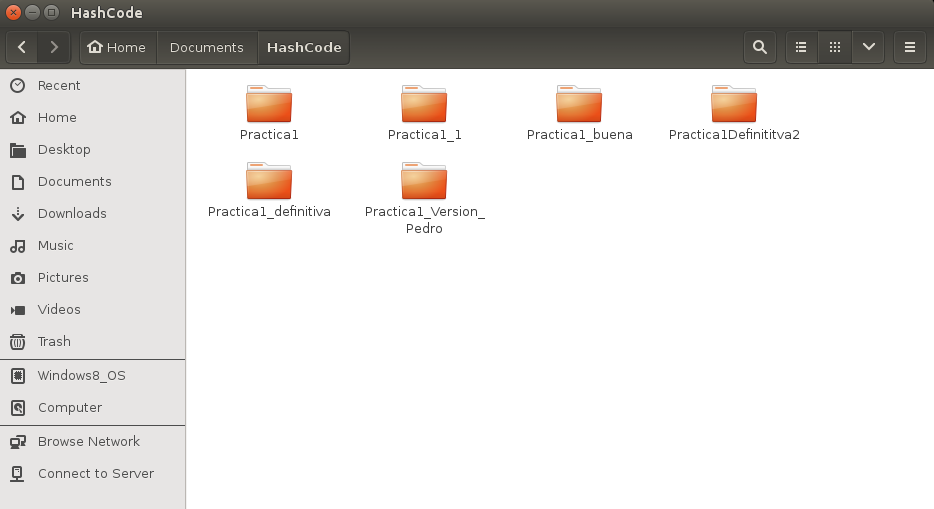
\includegraphics[height = 150pt]{dropboxClassic.png}
\end{figure}
\end{frame}

\begin{frame}
\frametitle{¿Por qué usar Git?}

Y porque a todos nos gusta ver
\begin{figure}[b]
\centering
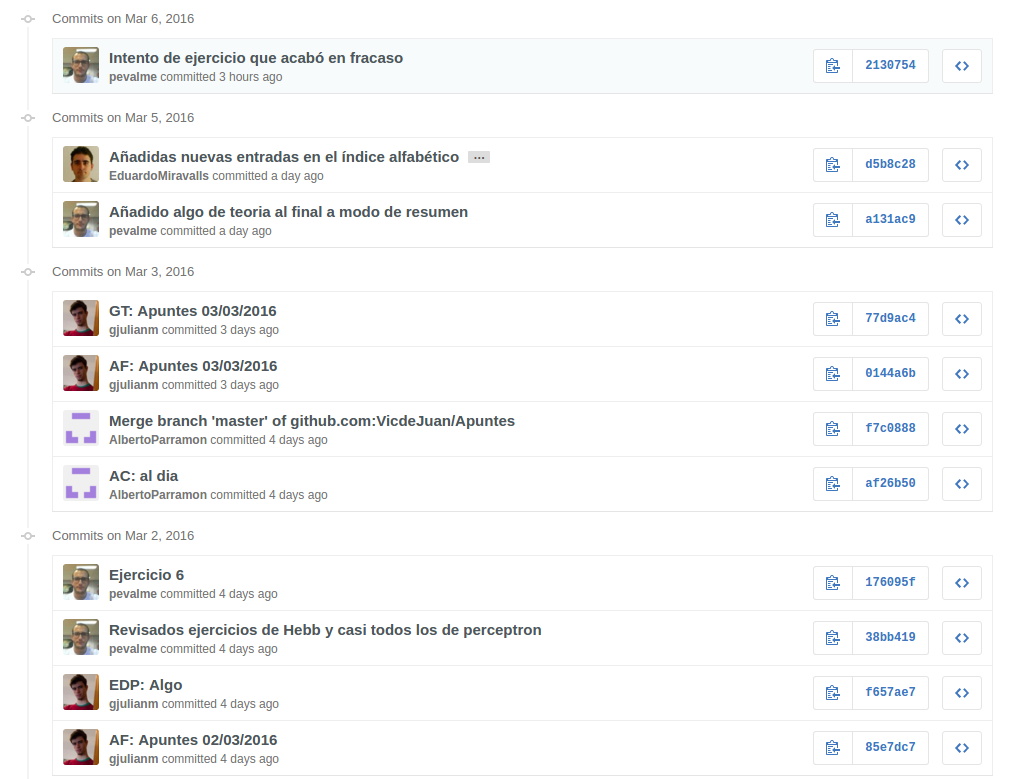
\includegraphics[height = 200pt]{gitCommits.png}
\end{figure}
\end{frame}

\section{¿Cómo funciona Git?}
\begin{frame}
\frametitle{Descripción informal}

\begin{figure}[b]
\centering
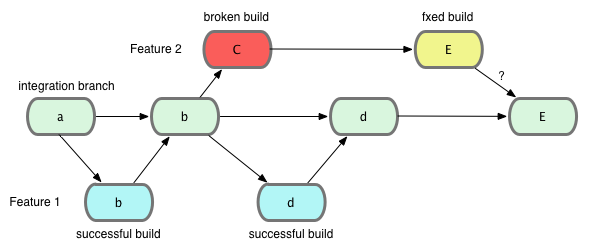
\includegraphics[height = 150pt]{gitProcess.png}
\end{figure}
\end{frame}

\begin{frame}
\begin{itemize}
\item Tenemos un proyecto en un servidor de Git. El proyecto se encuentra en el estado $A$.
\item Antes de empezar a trabjar debemos ``bajarnos'' el estado actual del proyecto.
\item Realizamos los cambios deseados hasta quedarnos satisfechos, llegando al estado $B$. Llega el momento de subir los cambios.
\begin{enumerate}
\item Cuando queremos actualizar los archivos del servidor, le decimos que el archivo que estaba en el estado $A$ queremos que pase al estado $B$.
\item Si el estado actual en el servidor es $A$, se actualiza con la versión $B$.
\item Si el estado actual en el servidor es otro distinto, $C$, comprueba si los camibos que implicó $C$ sobre $A$ son conflictivos con los que implica $B$. En caso afirmativo te avisa. En caso negativo, actualiza $C$ con lo que le faltase de $B$.
\end{enumerate}
\end{itemize}

\end{frame}

\section{Comandos de Git}
\begin{frame}
\frametitle{Comandos principales}
Vamos a ver los comandos más habituales en Git, aquellos que se usan \textit{constantemente} en el día a día.

Estos cambios permiten llevar a cabo las acciones descritas en el apartado anterior así como descartar cambios realizados en local.

No obstante, como hemos dicho al principio, Git guarda el histórico de los cambios y pueden realizarse muchísimas operaciones sobre este historial. No entraremos en ello por ahora pero es realmente interesante. \textbf{Git tiene un enorme potencial más allá de estas transparencias}
\end{frame}

\begin{frame}
\begin{enumerate}
\item \textbf{pull} Descarga los cambios del servidor a nuestra máquina.
\item \textbf{add} En local considera los cambios realizados en un fichero.
\item \textbf{commit} Prepara los cambios para ser subidos al repositorio. Permite además añadir comentarios.
\item \textbf{push} Sube los cambios al servidor.
\item \textbf{checkout} Descarta los cambios realizados en un fichero dejándolo en el estado en que se descargó.
\end{enumerate}

\begin{example}
git pull

git add fichero1.c include/fichero1.h

git commit -m ``Pila implementada''

git push

git checkout fichero2.c
\end{example}

\end{frame}

\section{Creamos un repositorio}
\end{document}
